\documentclass{meetings}


\usepackage{makecell}
\usepackage{xcolor}
\usepackage{multirow}
\usepackage{booktabs}
\usepackage{graphicx}
\usepackage{subcaption}
\usepackage{tikz}
\usetikzlibrary{positioning}

\definecolor{heading}{HTML}{002d57}



\usepackage[pages=all]{background}

\backgroundsetup{
scale=1,
color=black,
opacity=0.4,
angle=0,
contents={%
	
\includegraphics{background.pdf}
  }%
}




\setlength{\parskip}{0pt}
\setlength{\parindent}{0pt}
\setlength{\columnsep}{1cm}
\raggedcolumns


\author{S. König, L. Matzner, F. Rollbühler and J. Schmid}
\date{Tuesday, 20\textsuperscript{th} October 2020}

\newcommand{\todo}[1]{{\color{red}#1}}


\begin{document}
% Ich weiß, dass es die Beamer-Klasse gibt.
% Lasst mich doch alle in Ruhe!
% Die hier hatte ich noch rumliegen, das muss jetzt reichen.
\section{Motivation and Goal}
\sffamily
\begin{center}
	
	\vfill

	\begin{itemize}
		\item graph processing becomes increasingly important in academic and industrial environments
		\item many problems modeled with graphs, e.\,g.,\xspace machine learning and data mining
		\item many business models are based on graphs, e.\,g.,\xspace viral marketing or Google’s search engine
		\item graph sizes increase to several billion edges 
		\item[$\rightarrow$] performance, parallelism and distribution of graph algorithms becomes more important
	\end{itemize}

	\vfill

	\begin{minipage}{0.6\linewidth}
		\centering
		Main Goal: \itshape  Comparison of five graph processing systems in their performance on different graphs and algorithms.
	\end{minipage}

	\vfill
\end{center}


\section{Overview}
{\large
\begin{enumerate}
	\item Preliminaries
	\begin{itemize}
	\item Basics
	\item Computation Styles
	\item Hugepages
	\end{itemize}
	\item Frameworks
	\item Evaluation
	\begin{itemize}
	\item Research vs. Production Case
	\item Results
	\end{itemize}
	\item Conclusion and Outlook
\end{enumerate}
}
% In the past years several graph processing systems emerged.
% Graphs are growing fast and are becoming increasingly popular. Many problems can be modeled and solved using graphs.





\clearpage
\section{Preliminaries}
\begin{multicols}{2}
	\subsection*{Graphs}
	A \emph{weighted, directed graph} is the tuple $G=(V,E,w)$ where the \emph{vertex set} is $V\subseteq\mathbb N$ and the $E$ is the \emph{edge set} with
	\begin{equation*}
	  E\subseteq\{(x,y)\,|\, x,y\in V, x\neq y\}
	\end{equation*}
	and $w:E\rightarrow \mathbb R$ is a mapping of edge to a weight.
	
	\begin{center}
	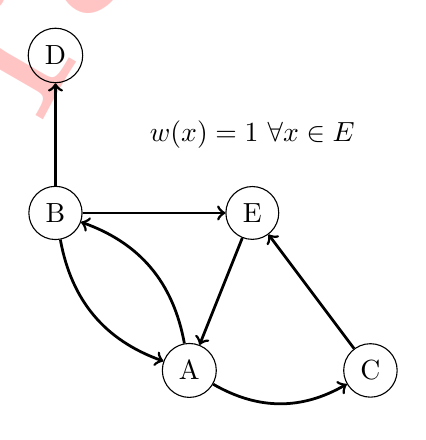
\begin{tikzpicture}
		\node[circle, draw] (a) at (1.7,0) {A};
		\node[circle, draw] (b) at (0,2) {B};
		\node[circle, draw] (c) at (4,0) {C};
		\node[circle, draw] (d) at (0,4) {D};
		\node[circle, draw] (e) at (2.5,2) {E};

		\draw[->, bend right, line width=1pt] (a) edge (b);
		\draw[->, bend right, line width=1pt] (a) edge (c);

		\draw[->, bend right, line width=1pt] (b) edge (a);
		\draw[->, line width=1pt] (b) edge (d);
		\draw[->, line width=1pt] (b) edge (e);

		\draw[->, line width=1pt] (c) edge (e);

		\draw[->, line width=1pt] (e) edge (a);

		\node at (2.5,3) {$w(x)=1\ \forall x\in E$};
	\end{tikzpicture}
	\end{center}
	\columnbreak
	\subsection*{Algorithms}
	\begin{description}
		\item[Single-Source Shortest-Paths (SSSP):] find the shortest path from a starting vertex to every other vertex

		\item[Breadth-first search (BFS):] find a node outgoing from a starting vertex, by increasing maximum hop count step-wise

		\item[PageRank (PR):] link analysis algorithm; weighs vertices, measuring their relative importance
	\end{description}
\end{multicols}


\clearpage
\begin{multicols}{2}
\section{Push Style}
\begin{center}
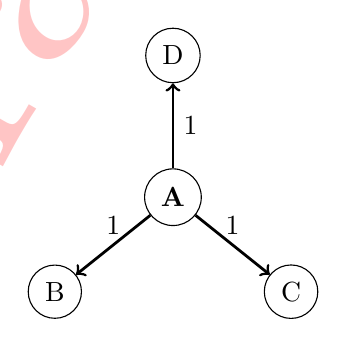
\begin{tikzpicture}
	\node[circle, draw] (a) at (1.5,1.2) {\bf A};
	\node[circle, draw] (b) at (0,0) {B};
	\node[circle, draw] (c) at (3,0) {C};
	\node[circle, draw] (d) at (1.5,3) {D};

	\draw[->, line width=1pt] (a) edge node[midway, above] {1} (b);
	\draw[->, line width=1pt] (a) edge node[midway, above] {1} (c);
	\draw[->, line width=1pt] (a) edge node[midway, right] {1} (d);
\end{tikzpicture}
\end{center}
\begin{itemize}
	\item reads active vertex, writes neighborhood 
	\item more efficient, if only few active vertices at the same time
	\item more efficient, if neighborhoods of active vertices do not overlap
\end{itemize}


\columnbreak
\section{Pull Style}
\begin{center}
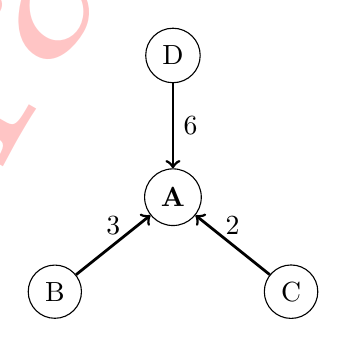
\begin{tikzpicture}
	\node[circle, draw] (a) at (1.5,1.2) {\bf A};
	\node[circle, draw] (b) at (0,0) {B};
	\node[circle, draw] (c) at (3,0) {C};
	\node[circle, draw] (d) at (1.5,3) {D};

	\draw[->, line width=1pt] (b) edge node[midway, above] {3} (a);
	\draw[->, line width=1pt] (c) edge node[midway, above] {2} (a);
	\draw[->, line width=1pt] (d) edge node[midway, right] {6} (a);
\end{tikzpicture}
\end{center}
\begin{itemize}
	\item reads neighborhood, writes active vertex
	\item[$\rightarrow$] only one write and many read operations
	\item less synchronization in parallel implementations needed
	\item more efficient, if many vertices active at the same time
\end{itemize}
\end{multicols}





\section{Hugepages}
\vspace{2cm}
\begin{itemize}
	\item most systems use virtual memory management
\begin{itemize}
	\item represents an abstraction to hardware memory
	\item virtual memory is organized in pages
	\item translations of virtual memory to physical memory are cached, because every translation takes time
\end{itemize}
	\item typically, memory pages are 4 KiB in size
	\item \textbf{hugepages} can be several MiB in size $\rightarrow$ reduce number of cache misses
	\item especially noticeable in very memory intensive applications
\end{itemize}








\definecolor{Galois}{HTML}{1f77b4}
\definecolor{Gemini}{HTML}{ff7f0e}
\definecolor{Giraph}{HTML}{2ca02c}
\definecolor{Ligra}{HTML}{d62728}
\definecolor{Polymer}{HTML}{9467bd}


\newgeometry{paperwidth=28.1cm, paperheight=18cm, left=2cm, right=2cm, top=0.7cm,bottom=1cm,includefoot,heightrounded}
\section{Frameworks}
\vfill
\renewcommand{\arraystretch}{1.2}
\begin{tabular}{lcccp{8cm}p{6cm}}
	Framework&Version&NUMA&Dist.&\multicolumn{1}{c}{Features}&\multicolumn{1}{c}{Notes}\\
	\toprule
	$\color{Galois}\blacksquare$\ \bf Galois&29.06.2020&\checkmark&(\checkmark)&general purpose library designed for parallel programming&Distributed using Gluon\\\midrule
	$\color{Gemini}\blacksquare$\ \bf Gemini&02.11.2016&\checkmark&\checkmark&distributed message-based approach from scratch&Version contains bugs that had to be fixed \\\midrule
	$\color{Giraph}\blacksquare$\ \bf Giraph&08.05.2020&X&\checkmark&built on Apache Hadoop&BFS is not natively supported \\\midrule
	$\color{Ligra}\blacksquare$\ \bf Ligra&14.08.2019&\checkmark&X&dynamically switches between push and pull style&\\\midrule
	$\color{Polymer}\blacksquare$\ \bf Polymer&28.08.2018&\checkmark&X&optimizes data layout and memory access strategies&\\
\end{tabular}
\vfill





\restoregeometry


\section{Evaluation}
\begin{multicols}{2}
\subsection*{Machines}
vsflash1-5, 
\begin{itemize}
	\item 96 cores, of which 48 virtual
	\item 256 GB of RAM each\footnote{\sffamily one machine only 128 GB}
	\item Ubuntu 18.04.2 LTS
\end{itemize}
\subsection*{Measurements}
\begin{itemize}
	\item \textbf{execution time}: time from start to finish of the console command
	\item \textbf{calculation time}: time the framework actually executed the algorithm
	%\item \textbf{overhead}: time difference between execution time and calculation time \newline (time to read the input graph, initialization, etc.) -- brauchen wir das überhaupt?
	\item executed each test case 10 times
\end{itemize}

\columnbreak

\subsection*{Graphs}
Both rMat graphs are synthetic, others are real-world data sets; Flickr: 24MB, rMat28: 76GB%
\begin{center}
	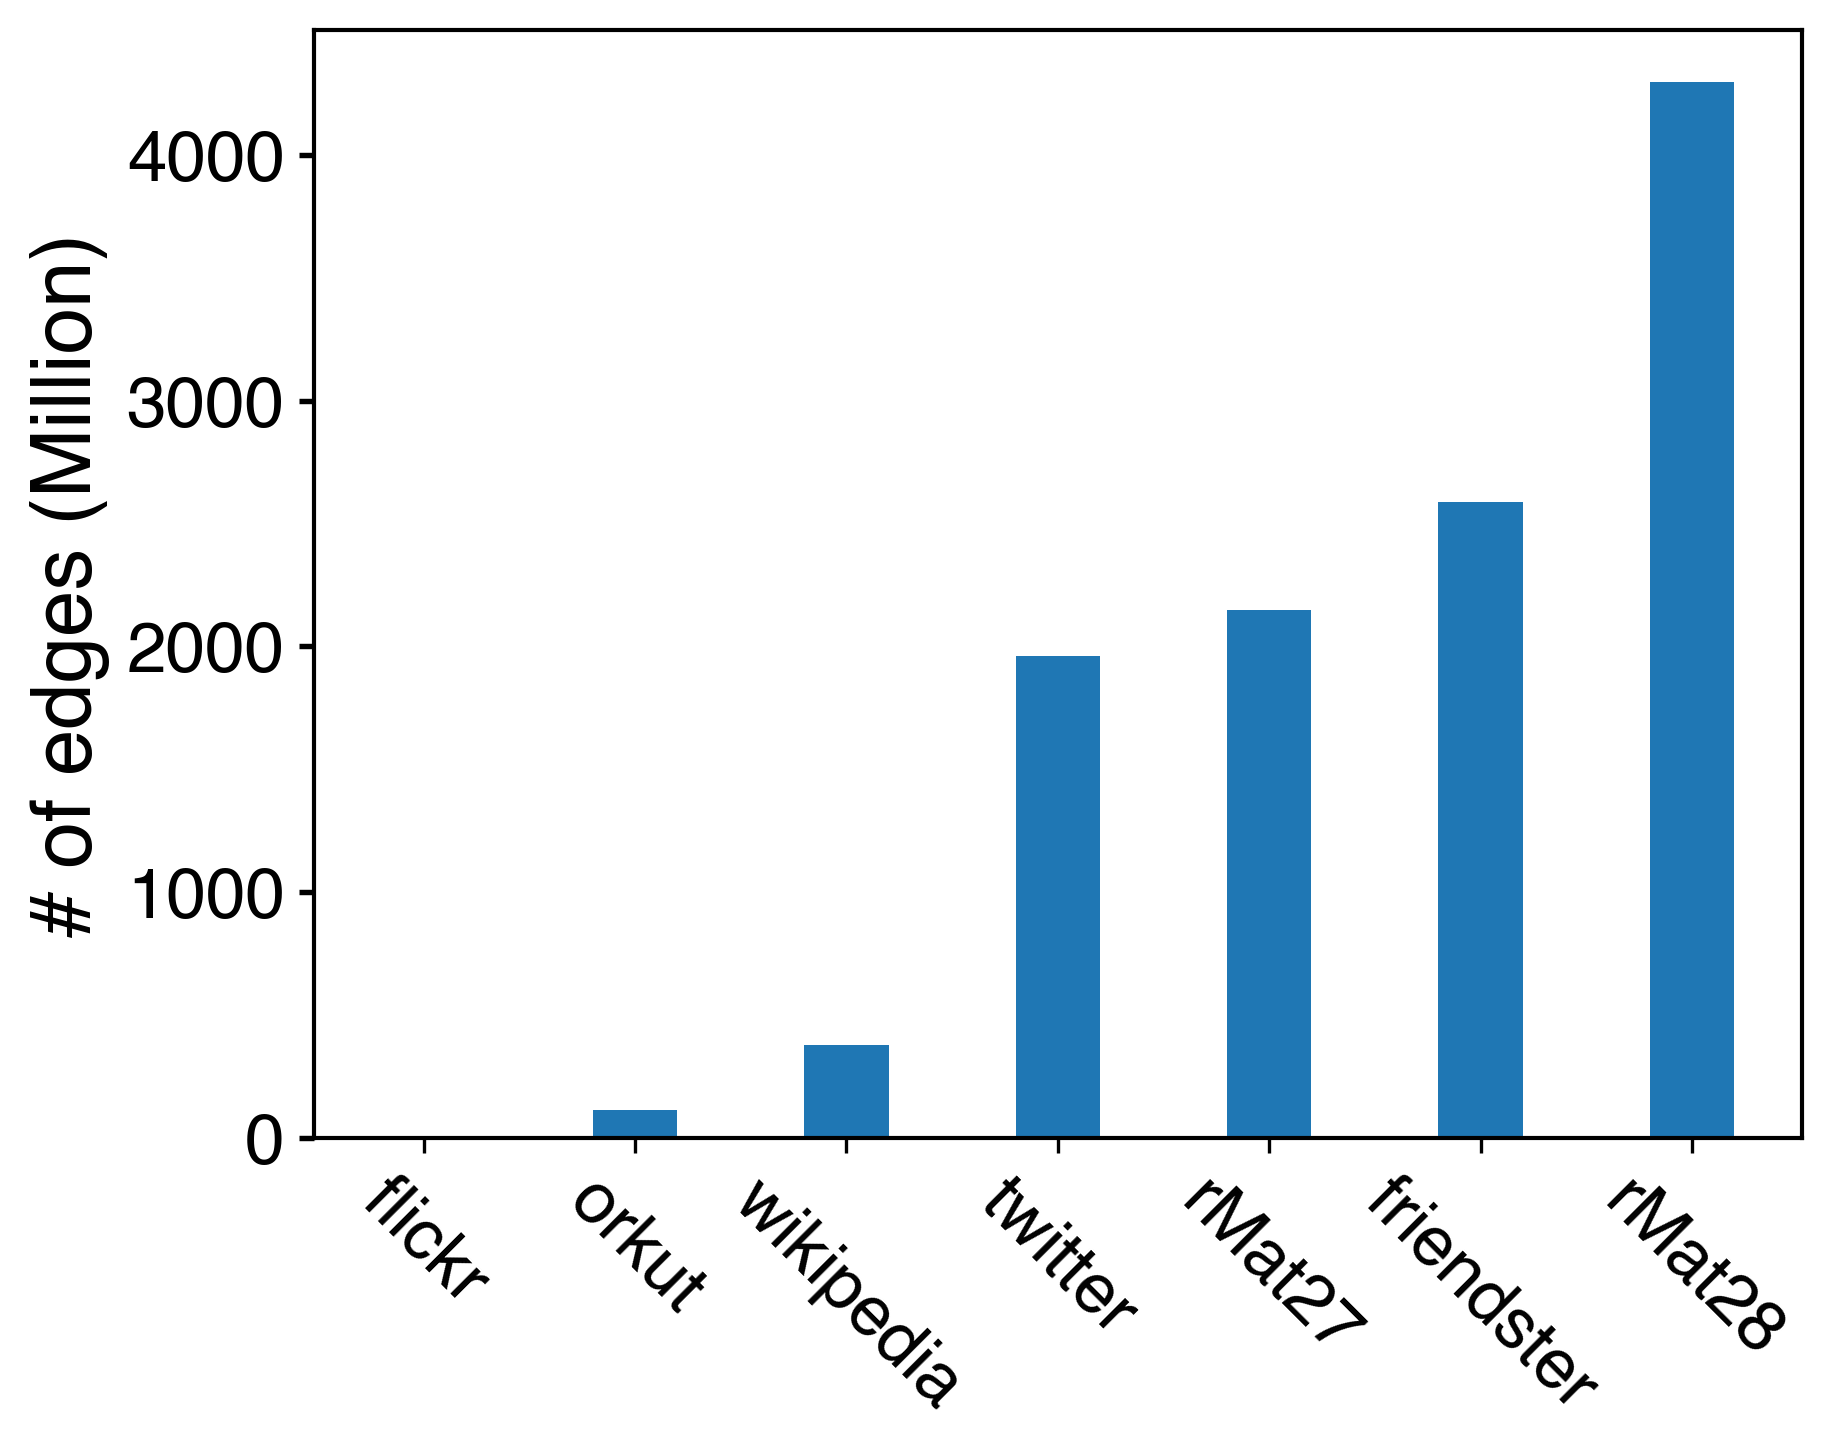
\includegraphics[width=\linewidth]{graphsize.png}
\end{center}
\end{multicols}


\begin{multicols}{2}
\section{Production Case}
\vspace{1cm}
\begin{itemize}
	\item running system: multiple calculations on a single graph
	\item graph data stays loaded between calculations
	\item[$\rightarrow$] short calculation times should be preferred
	\item Not main focus of this presentation!\footnote{\sffamily see paper for details}
\end{itemize}

\columnbreak
\section{Research Case}
\vspace{1cm}
\begin{itemize}
	\item individual calculation cases: possibly new graph for each calculation
	\item frequently changing algorithm
	\item[$\rightarrow$] framework should be relatively fast on different algorithms
	\item[$\rightarrow$] overall small execution times should be preferred
\end{itemize}
\end{multicols}


% \section{Production Case Single Node}

% \begin{figure}[h]
% 	\begin{subfigure}{0.32\textwidth}
% 		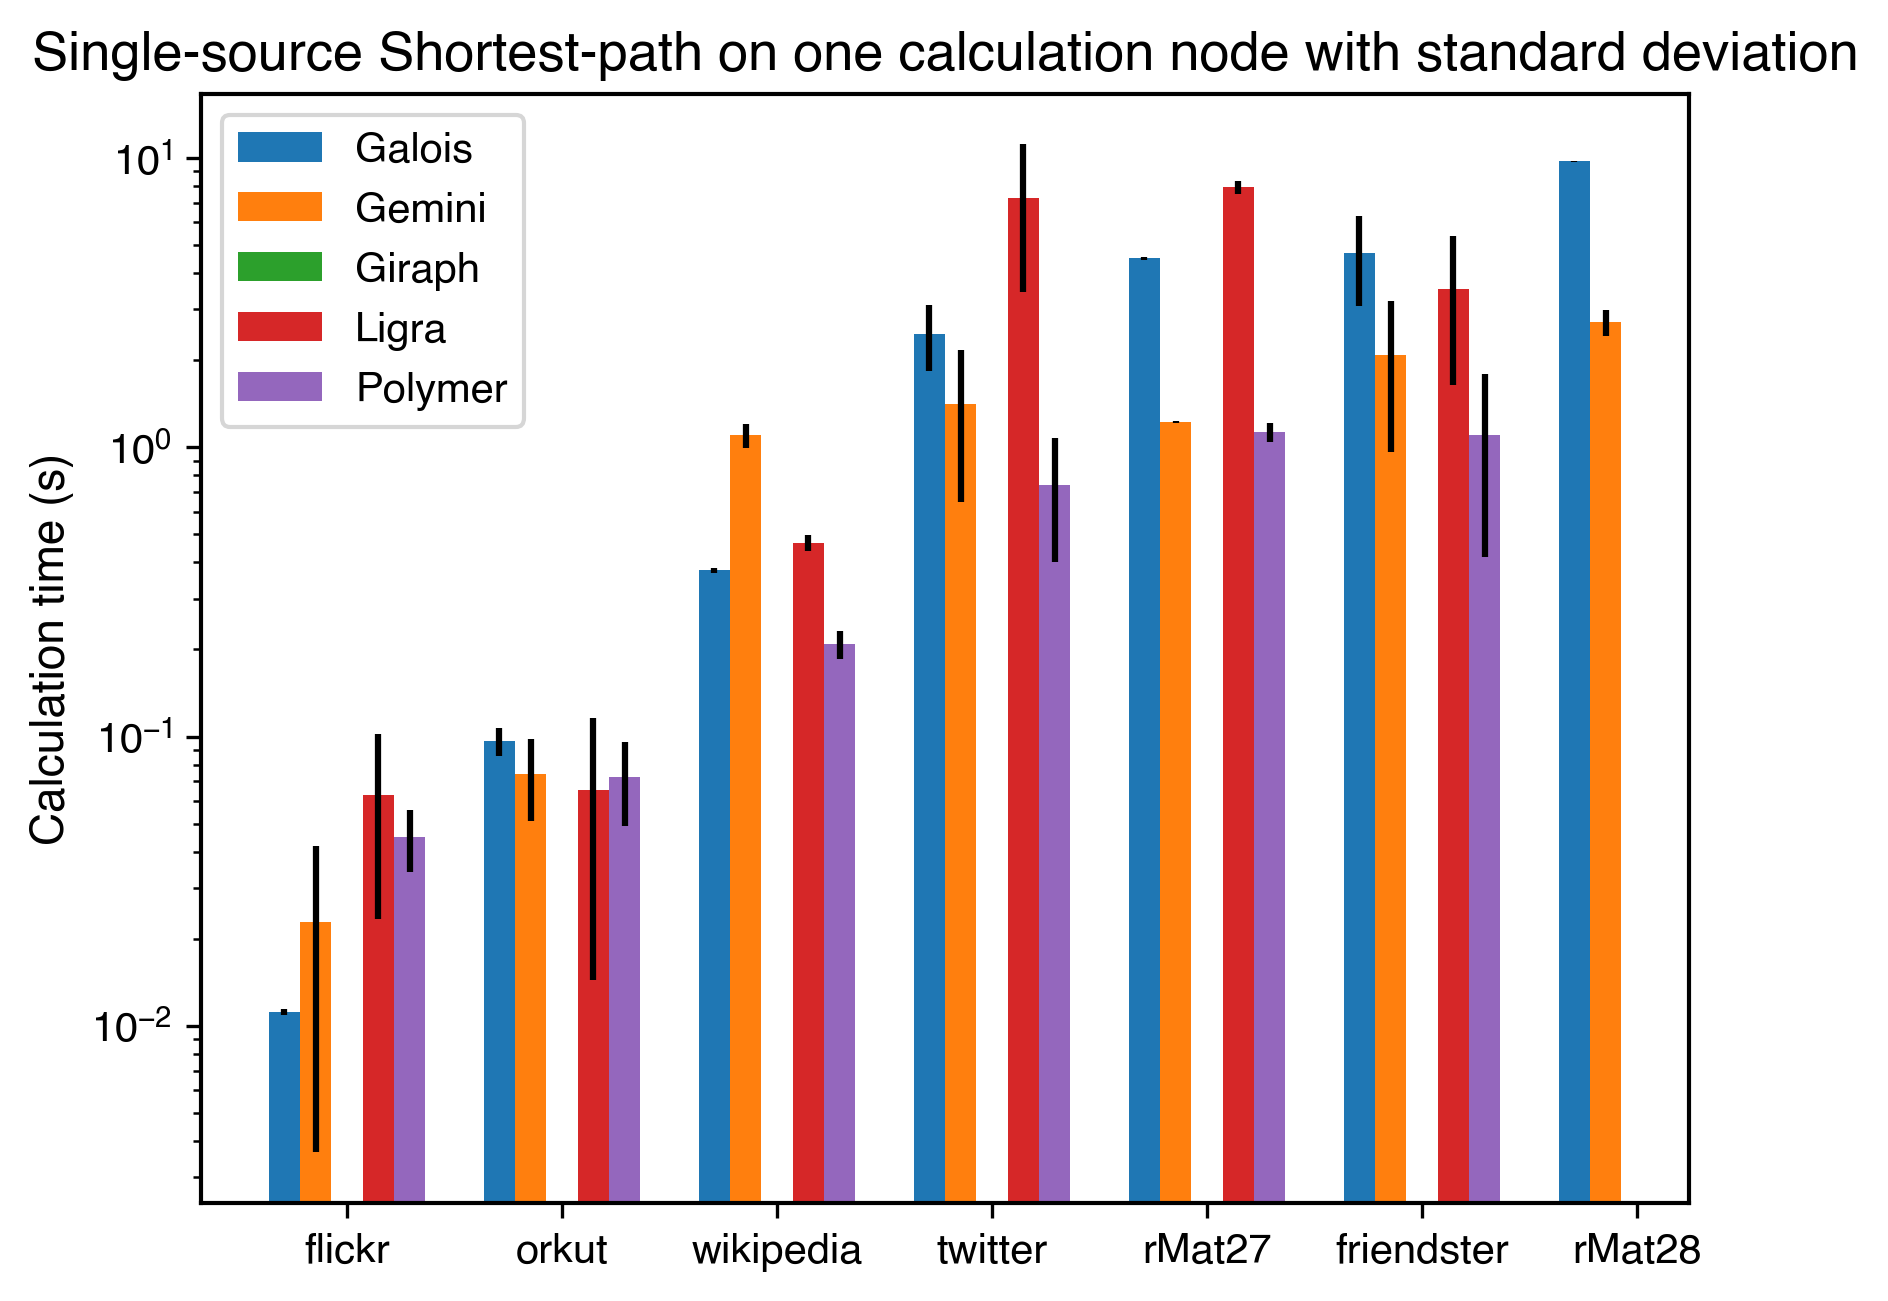
\includegraphics[width=\linewidth]{../../plots/singleNodeSSSP_calcTime.png}
% 		\caption{SSSP}
% 	\end{subfigure}
% 	\begin{subfigure}{0.32\textwidth}
% 		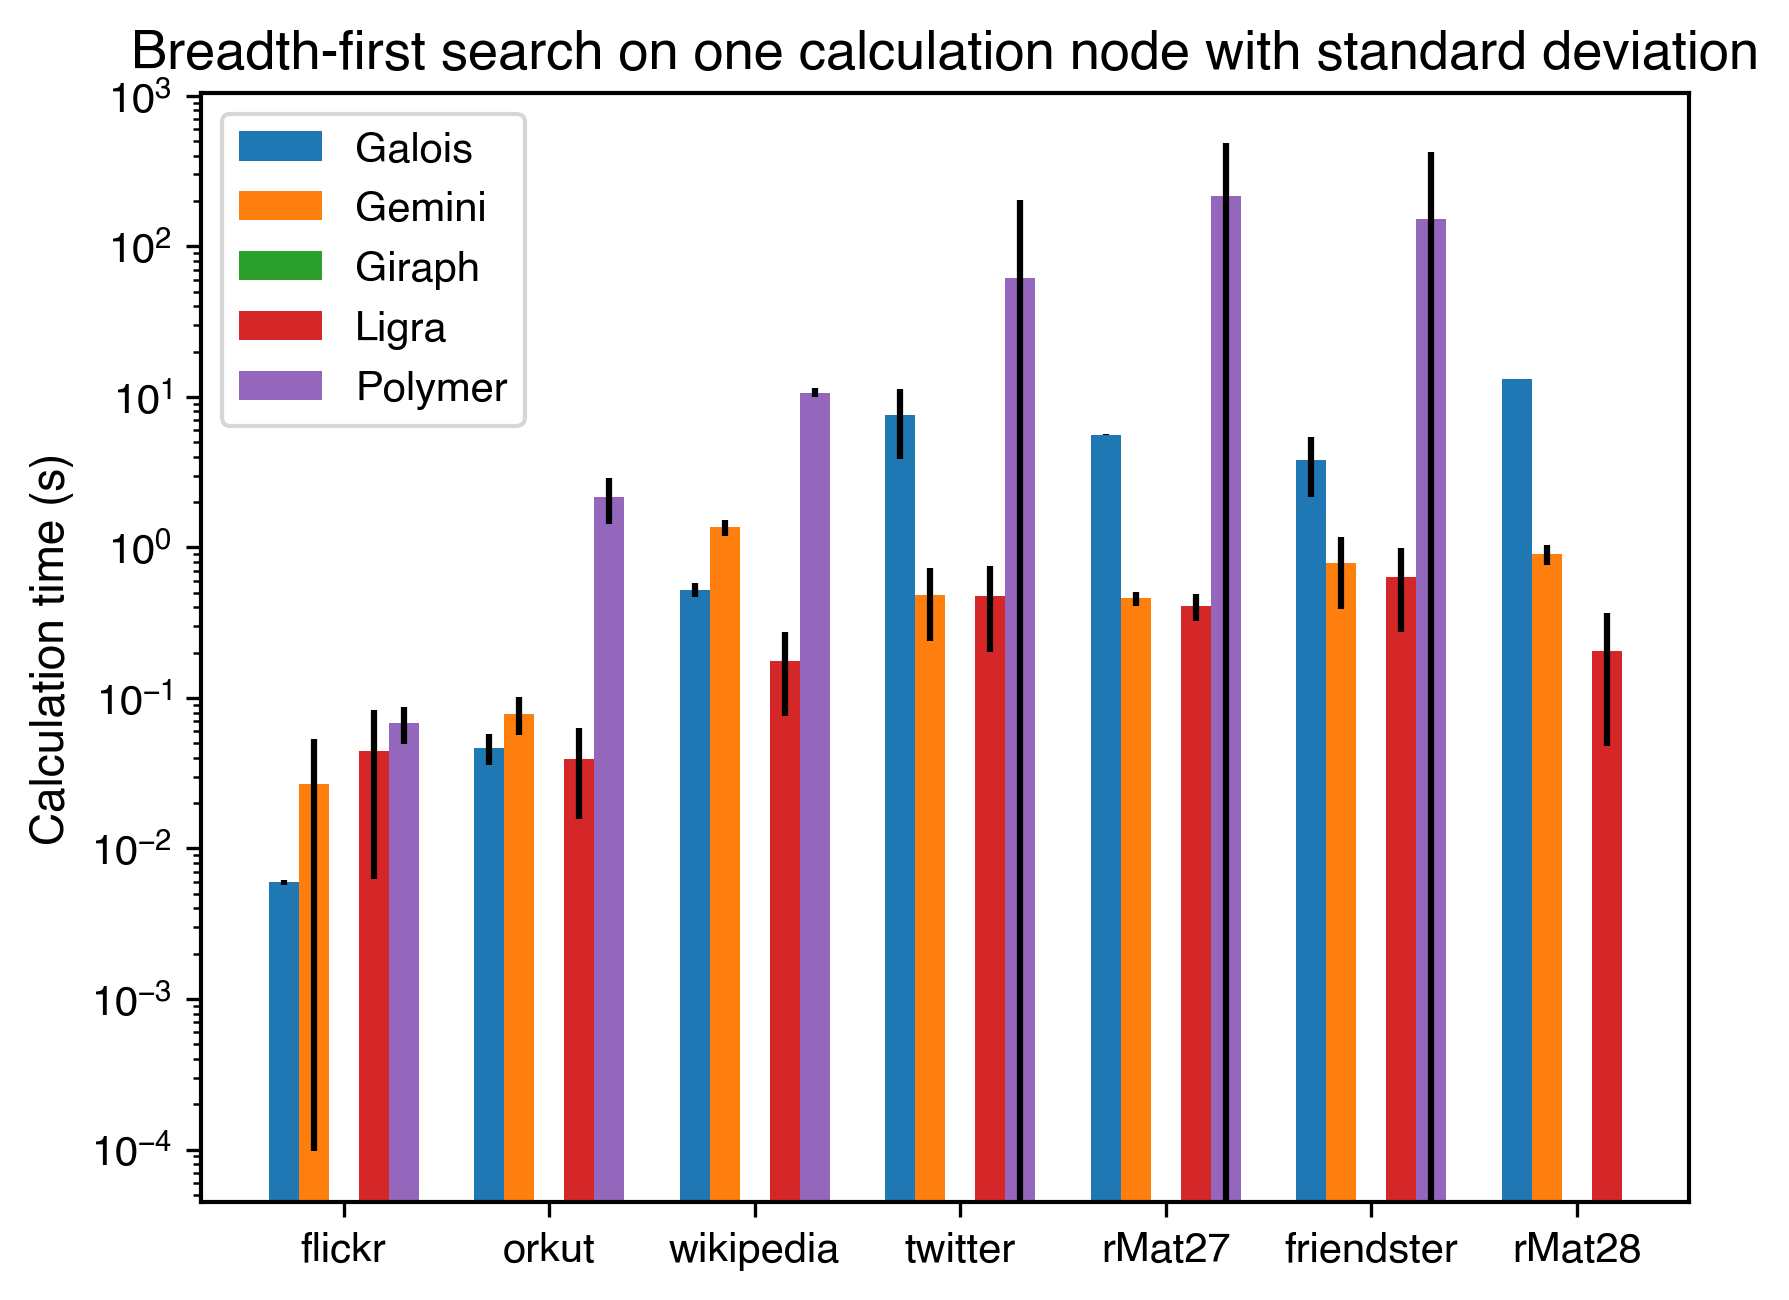
\includegraphics[width=\linewidth]{../../plots/singleNodeBFS_calcTime.png}
% 		\caption{BFS}
% 	\end{subfigure}
% 	\begin{subfigure}{0.32\textwidth}
% 		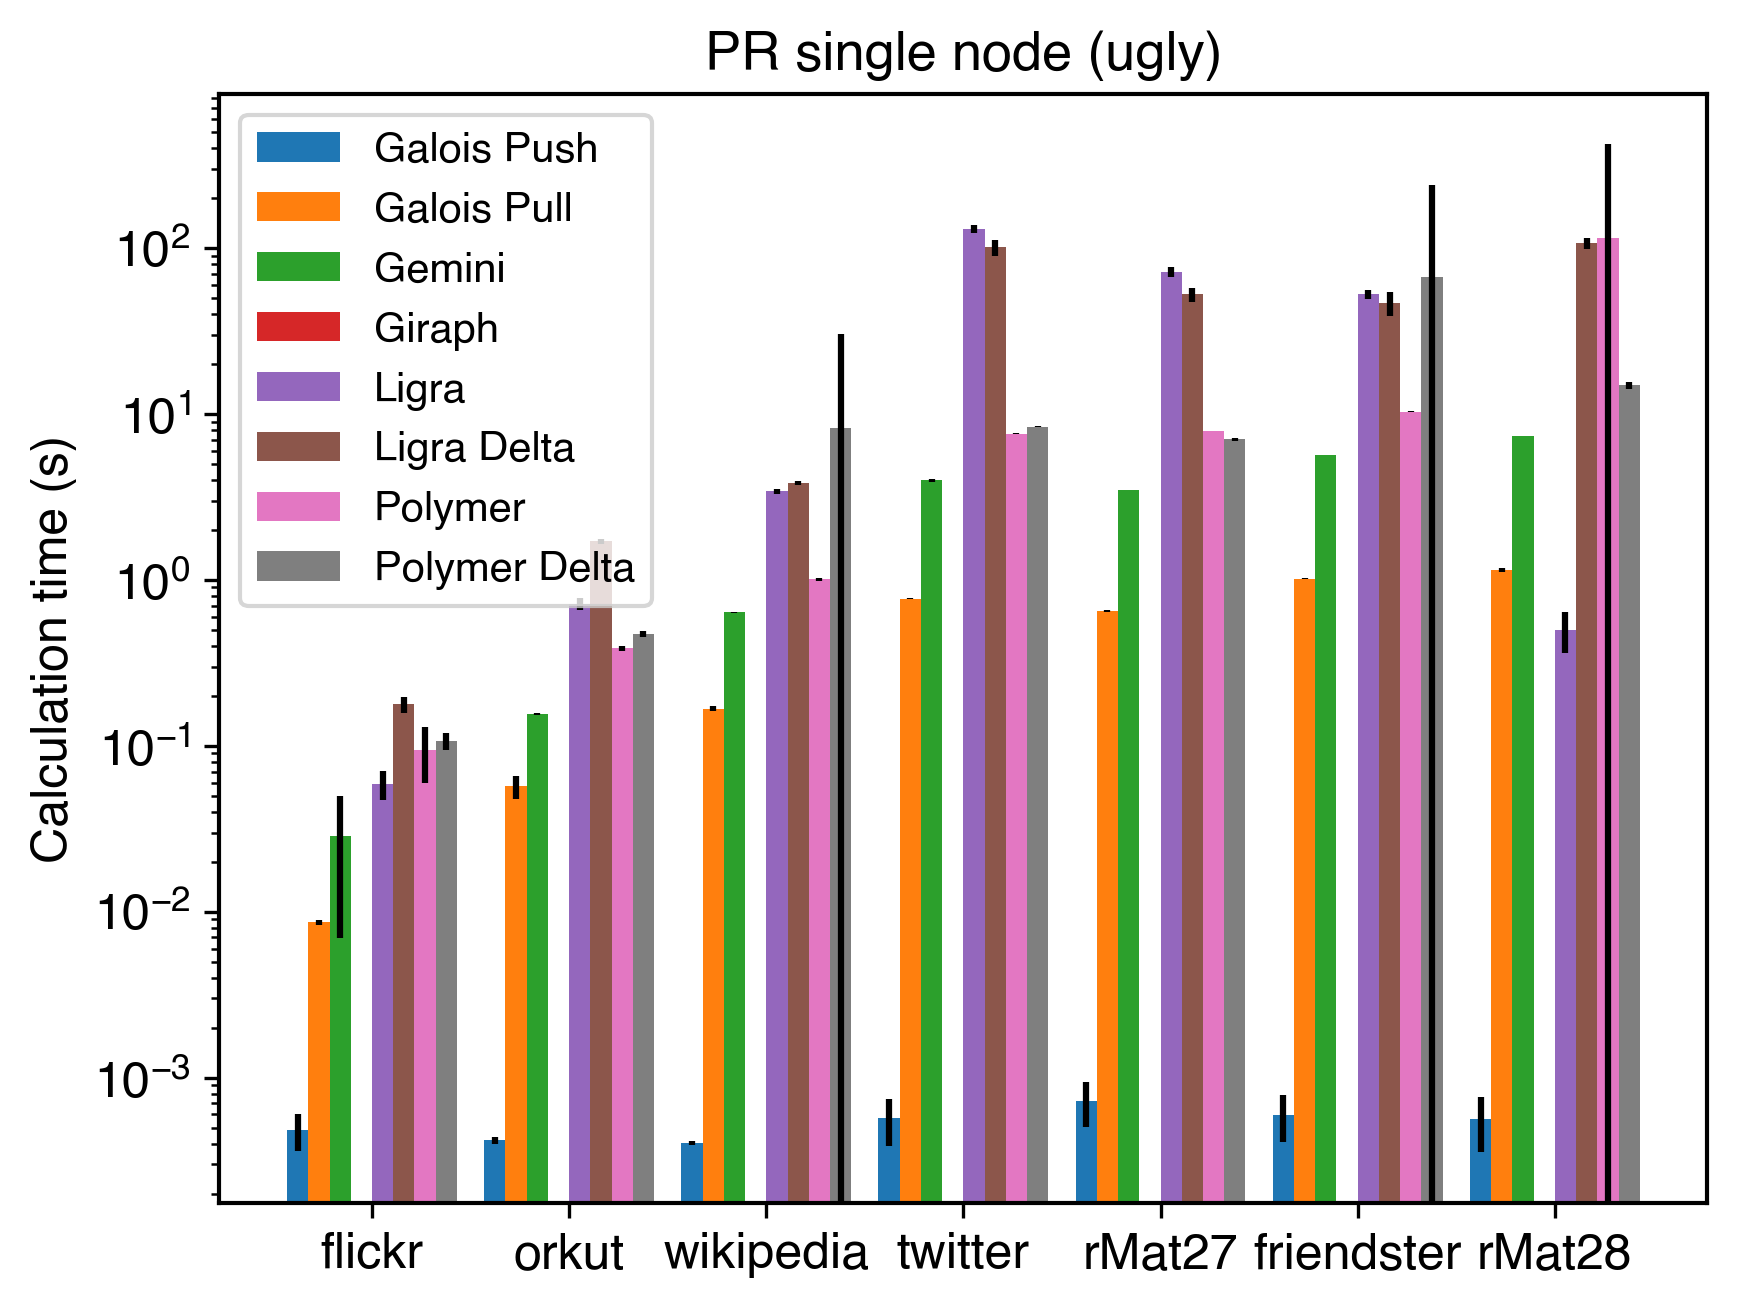
\includegraphics[width=\linewidth]{../../plots/singleNodePR_calcTime.png}
% 		\caption{PR}
% 	\end{subfigure}
% \end{figure}
% \begin{itemize}
% 	\item Giraph is either very slow or requires too much RAM (>256 GB)
% 	\item On SSSP, Polymer is fastest, followed by Gemini on second place
% 	\item On BFS, Gemini and Ligra are comparable and fastest on the larger graphs
% 	\item On PR, Galois Pull is fastest, we exclude Galois Push because of possible measuring errors.
% 	\item \todo{Message-based approach can compete with shared-memory}
% \end{itemize}
% \todo{Grafiken Größer?}


\section{Production Case Distributed}

\begin{figure}[h]
	\begin{subfigure}{0.45\textwidth}
		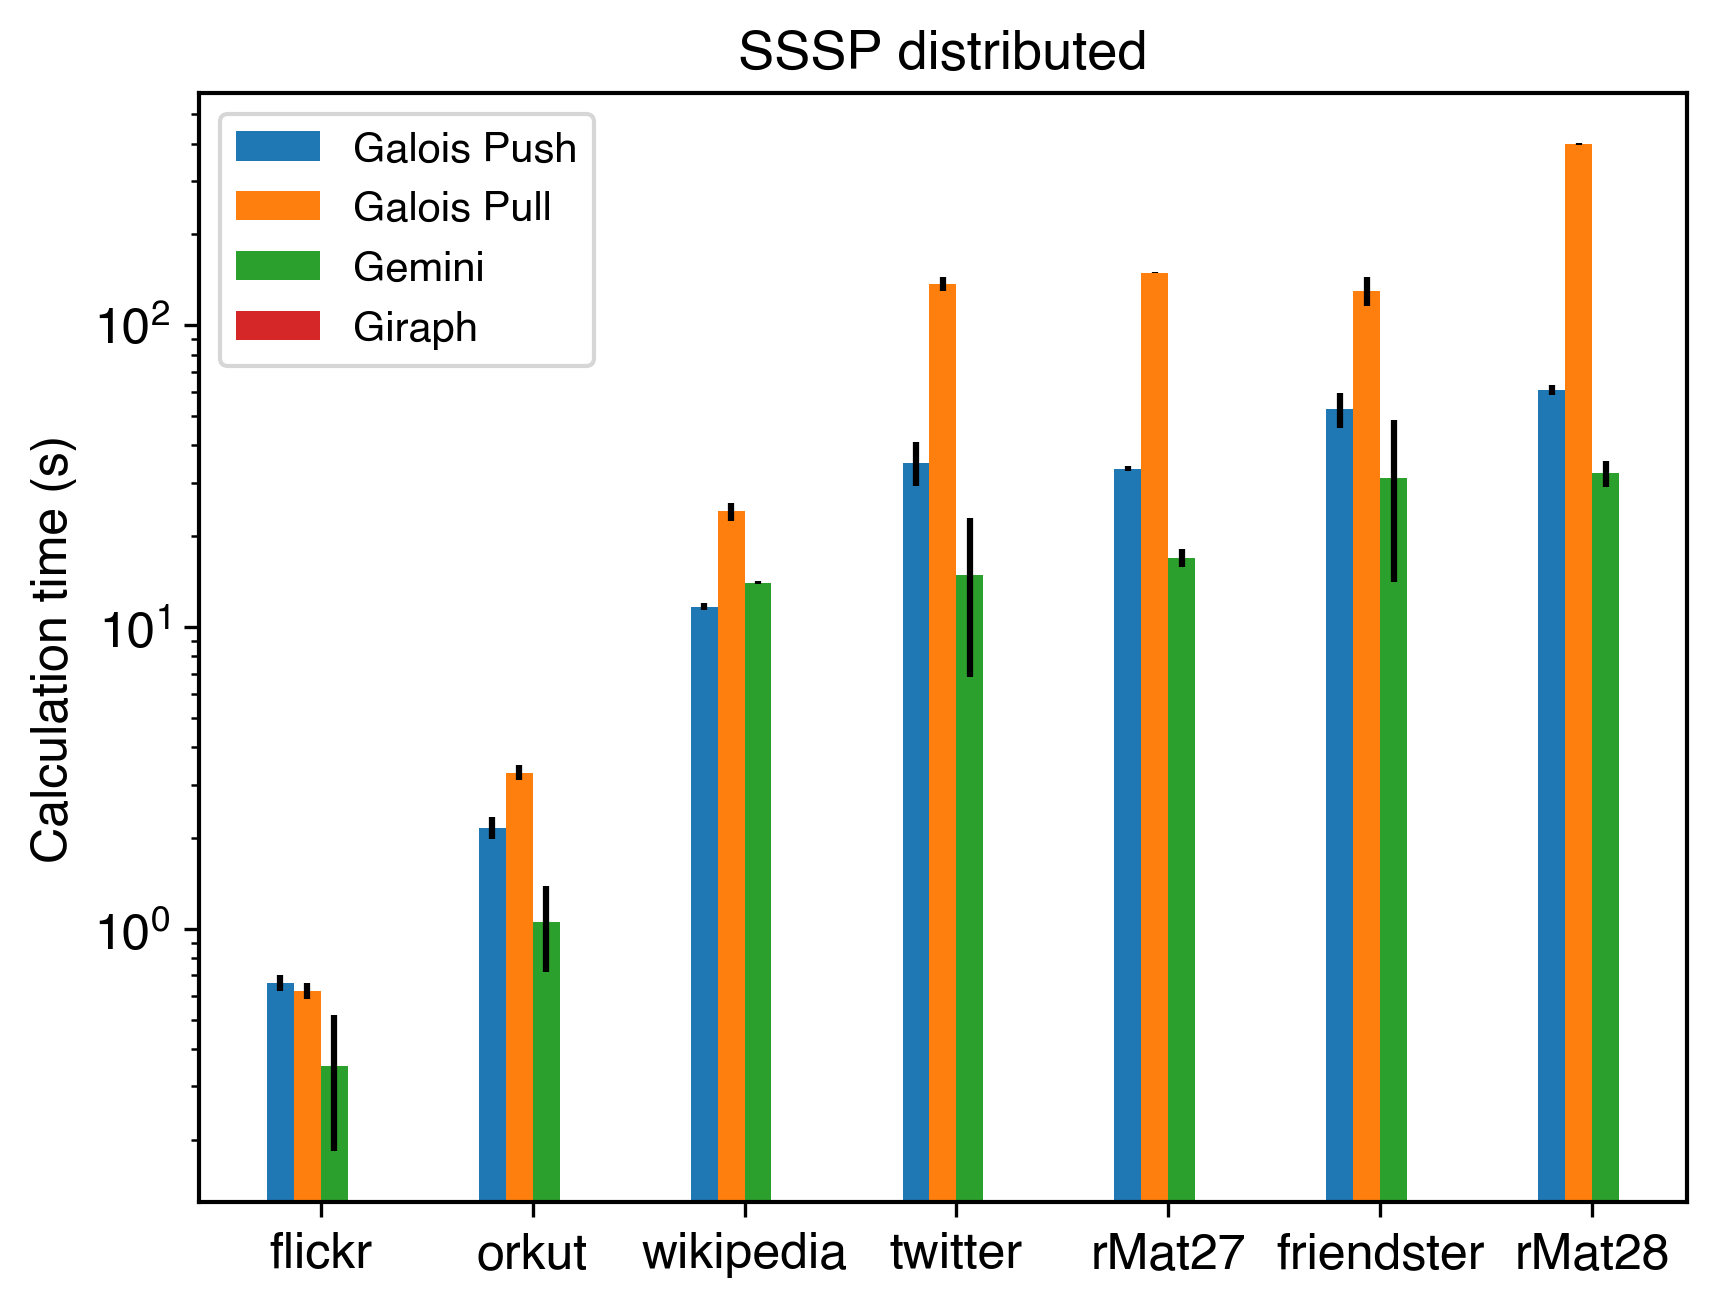
\includegraphics[width=\linewidth]{../../plots/distributedSSSP_calcTime.png}
		\caption{SSSP}
	\end{subfigure}
	\hfil
	\begin{subfigure}{0.45\textwidth}
		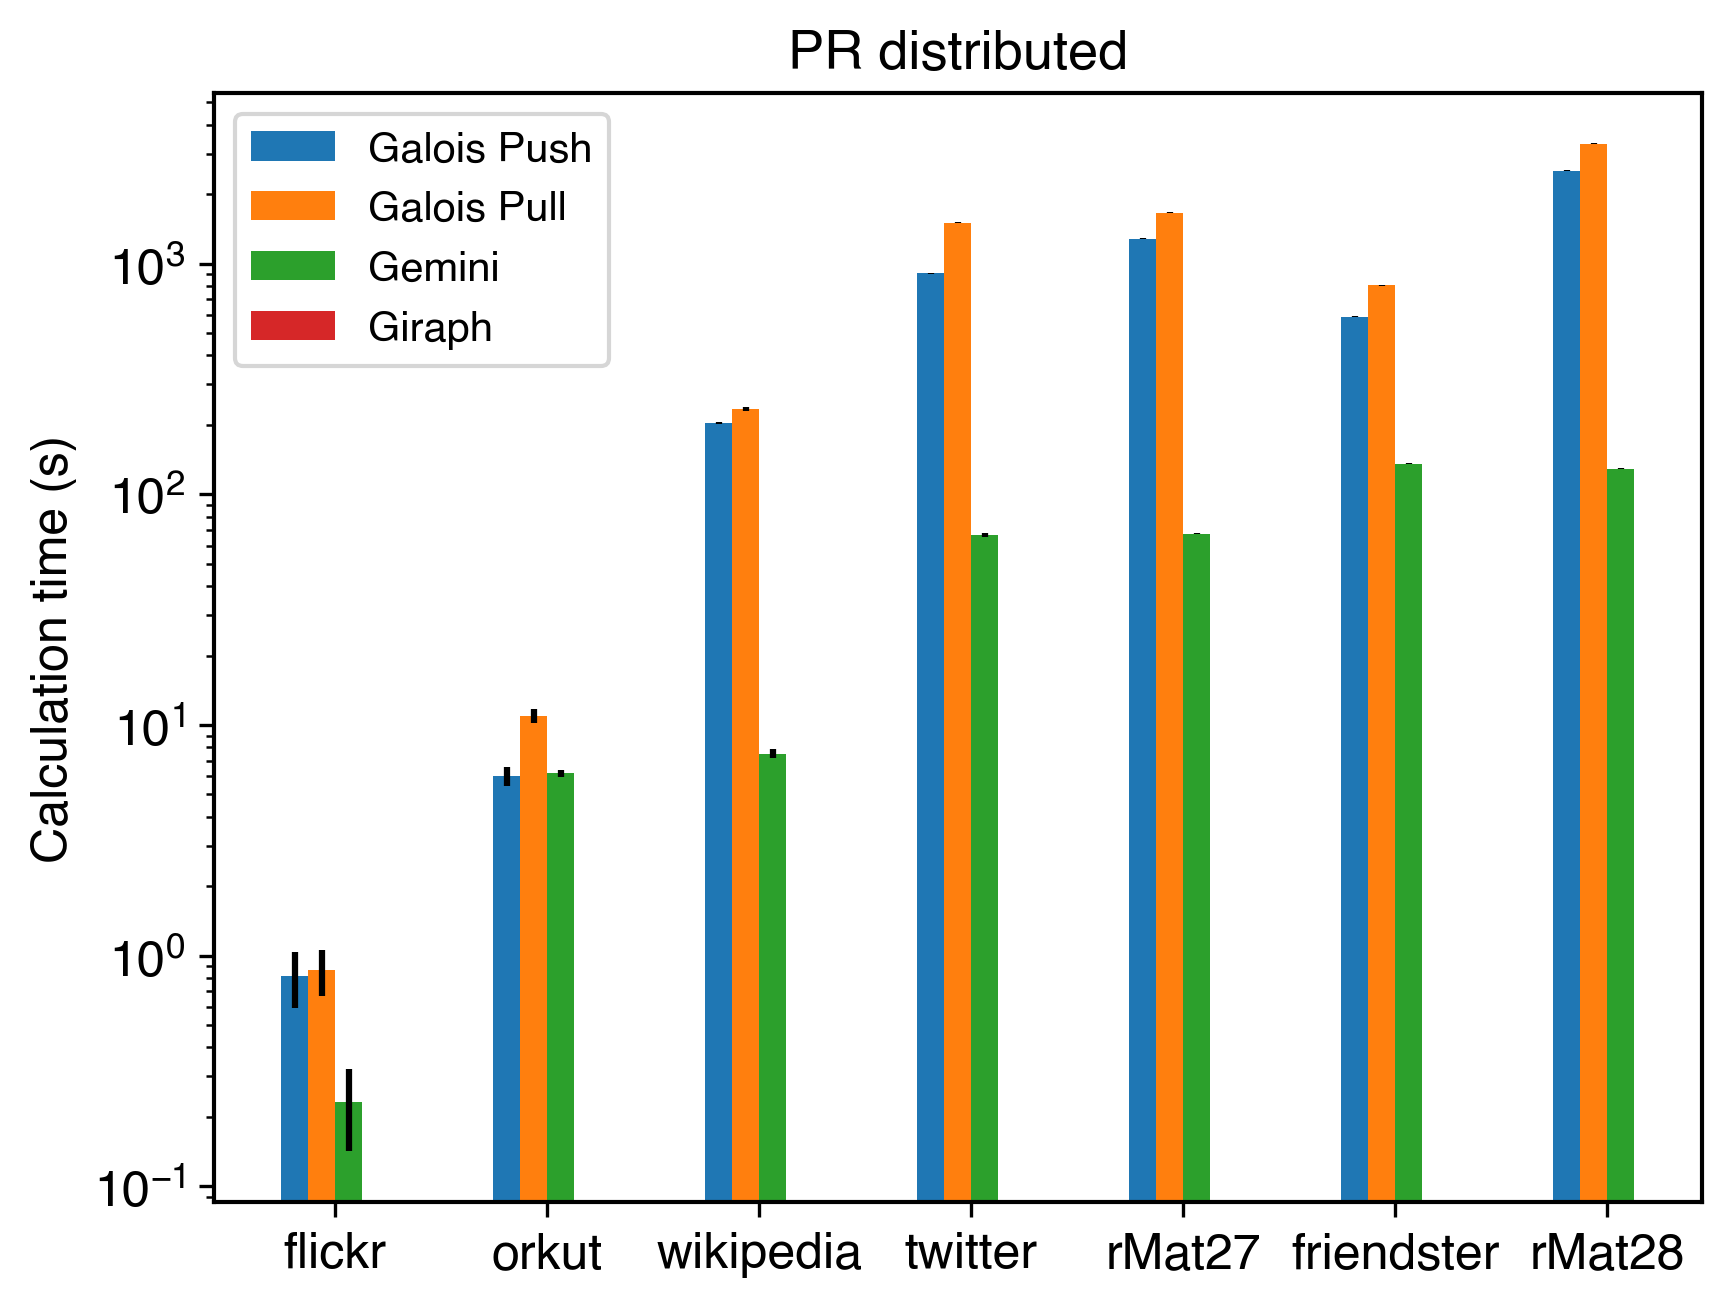
\includegraphics[width=\linewidth]{../../plots/distributedPR_calcTime.png}
		\caption{PR}
	\end{subfigure}
\end{figure}
\begin{itemize}
	\item Giraph is fastest on SSSP and BFS on the real world graphs
	\item Giraph has problems with synthetic graphs
	\item Gemini is fastest on PR, with Giraph on second place
\end{itemize}











\section{Research Case Single Node}

\begin{figure}[h]
	\begin{subfigure}{0.45\textwidth}
		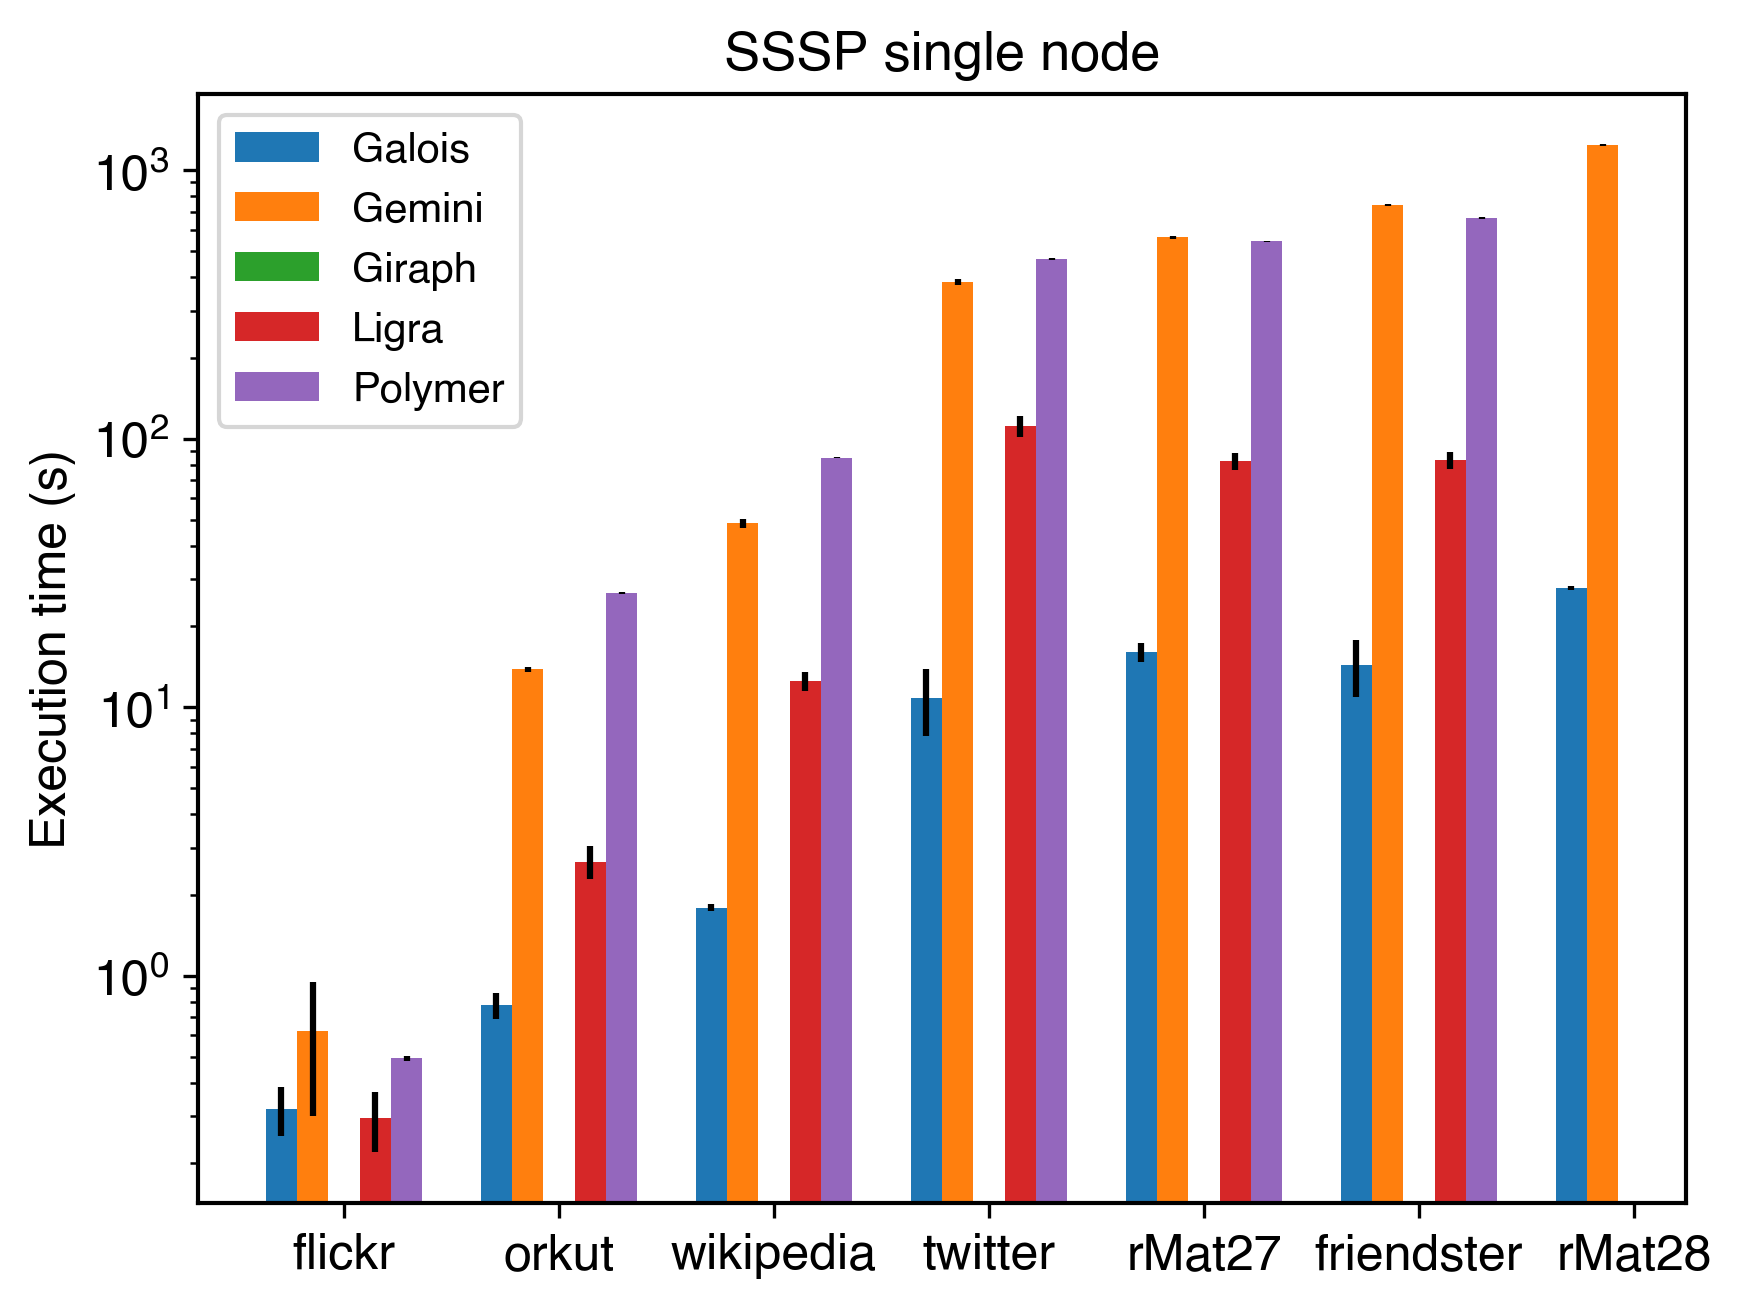
\includegraphics[width=\linewidth]{../../plots/singleNodeSSSP_execTime.png}
		\caption{SSSP}
		\label{fig:singleNodeSSSP_exec}
	\end{subfigure}
	\hfil
	\begin{subfigure}{0.45\textwidth}
		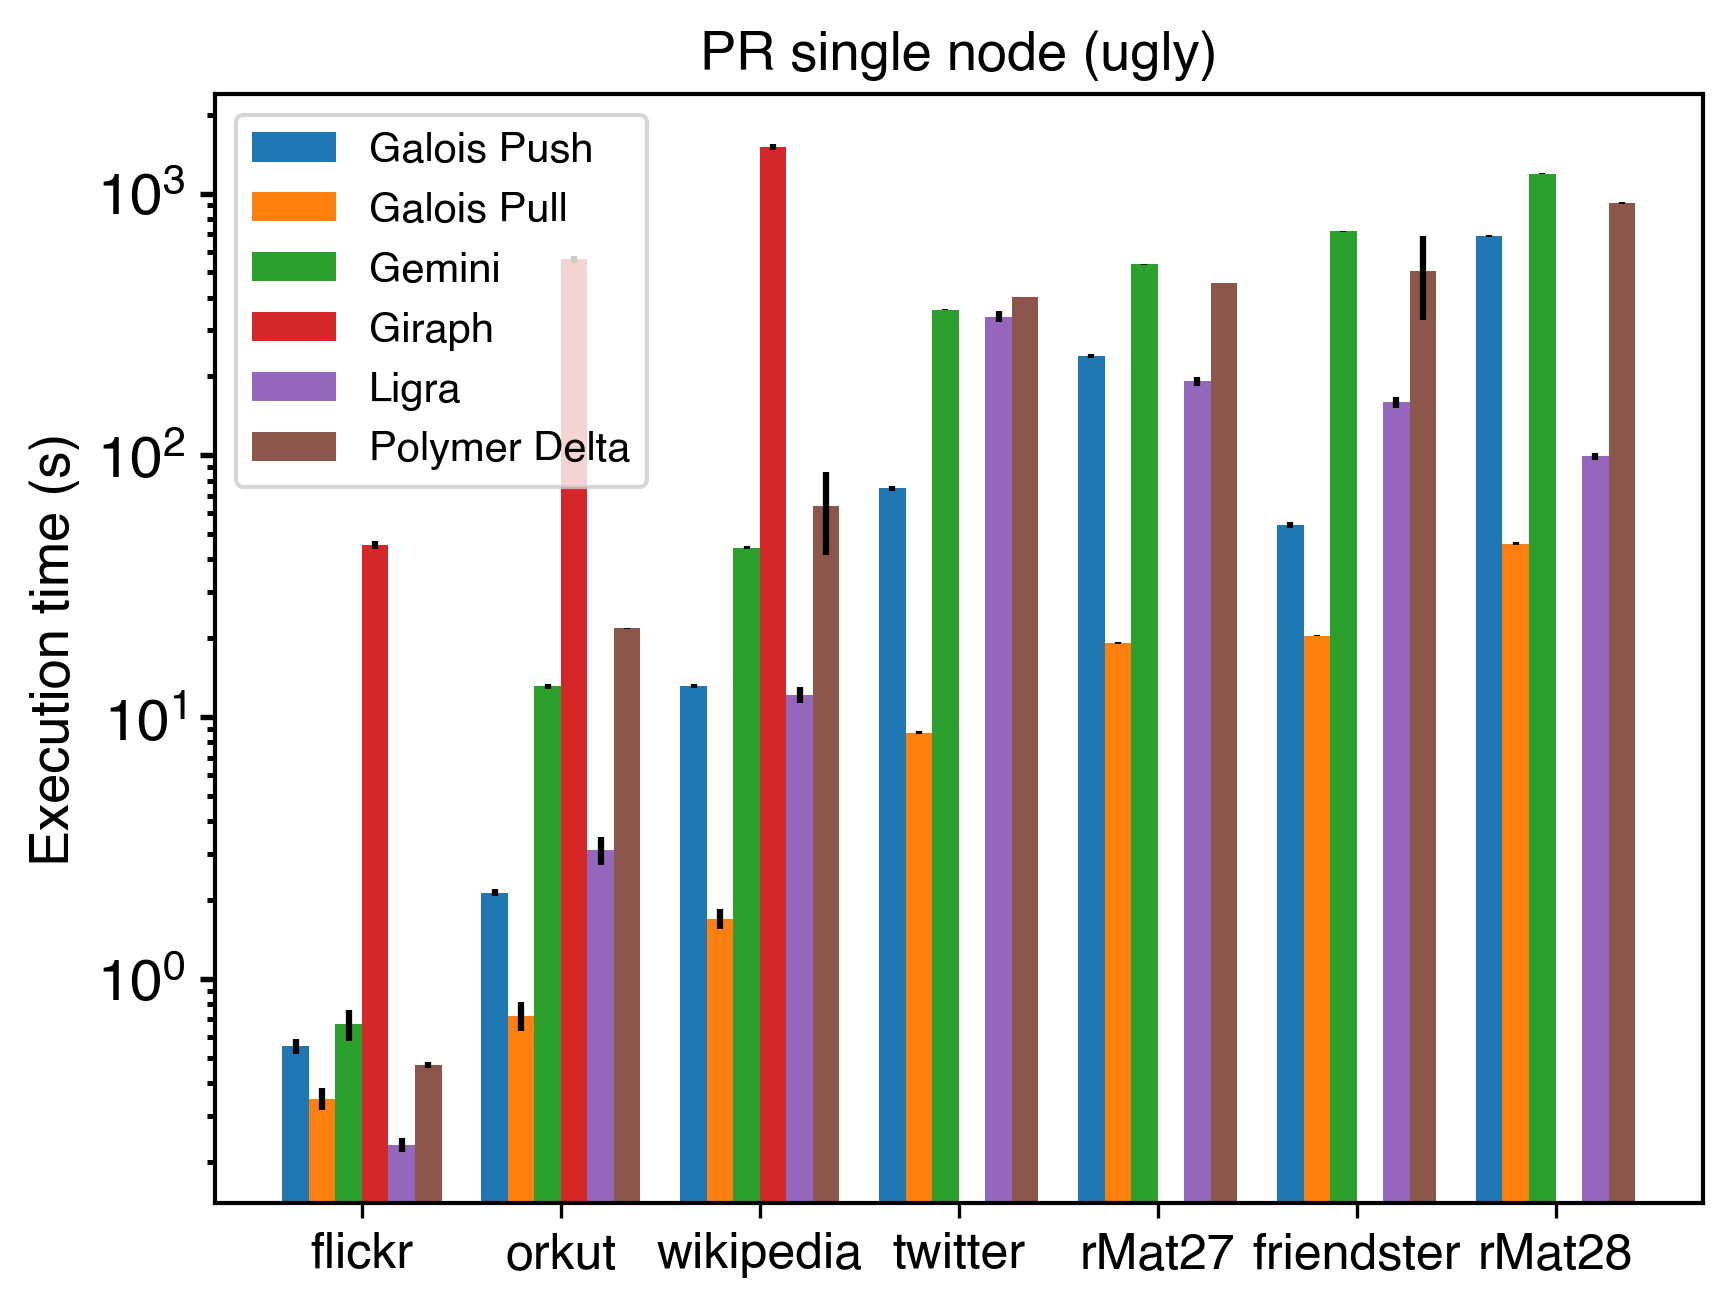
\includegraphics[width=\linewidth]{../../plots/singleNodePR_execTime.png}
		\caption{PR}
		\label{fig:singleNodeSSSP_exec}
	\end{subfigure}
\end{figure}
\begin{itemize}
	\item Giraph is either slowest or requires too much RAM (>256 GB)
	\item Galois is fastest in almost all cases, second fastest is Ligra
	\item Gemini and Polymer are comparably slow
\end{itemize}


\section{Research Case Distributed}

\begin{figure}[h]
	\begin{subfigure}{0.45\textwidth}
		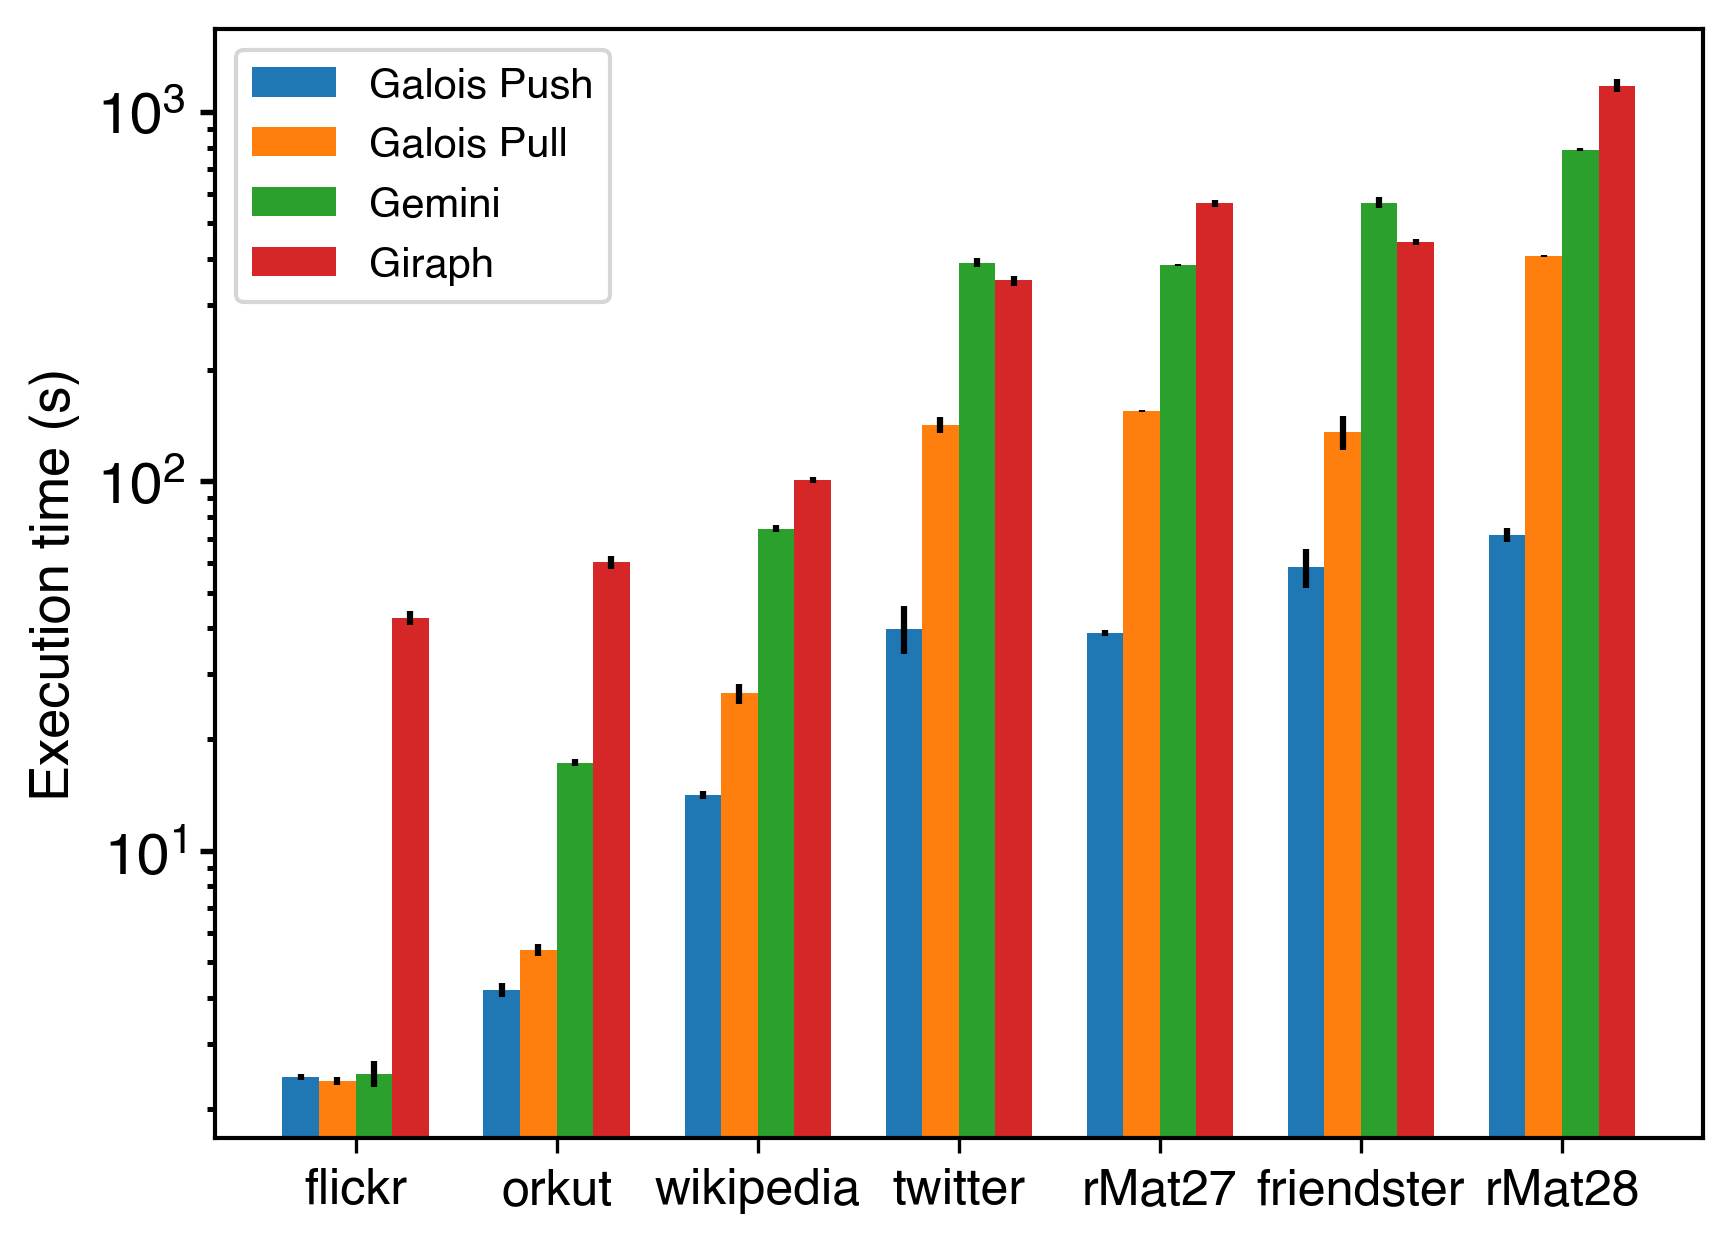
\includegraphics[width=\linewidth]{../../plots/distributedSSSP_execTime.png}
		\caption{SSSP}
		\label{fig:distributedSSSP_exec}
	\end{subfigure}
	\hfil
	\begin{subfigure}{0.45\textwidth}
		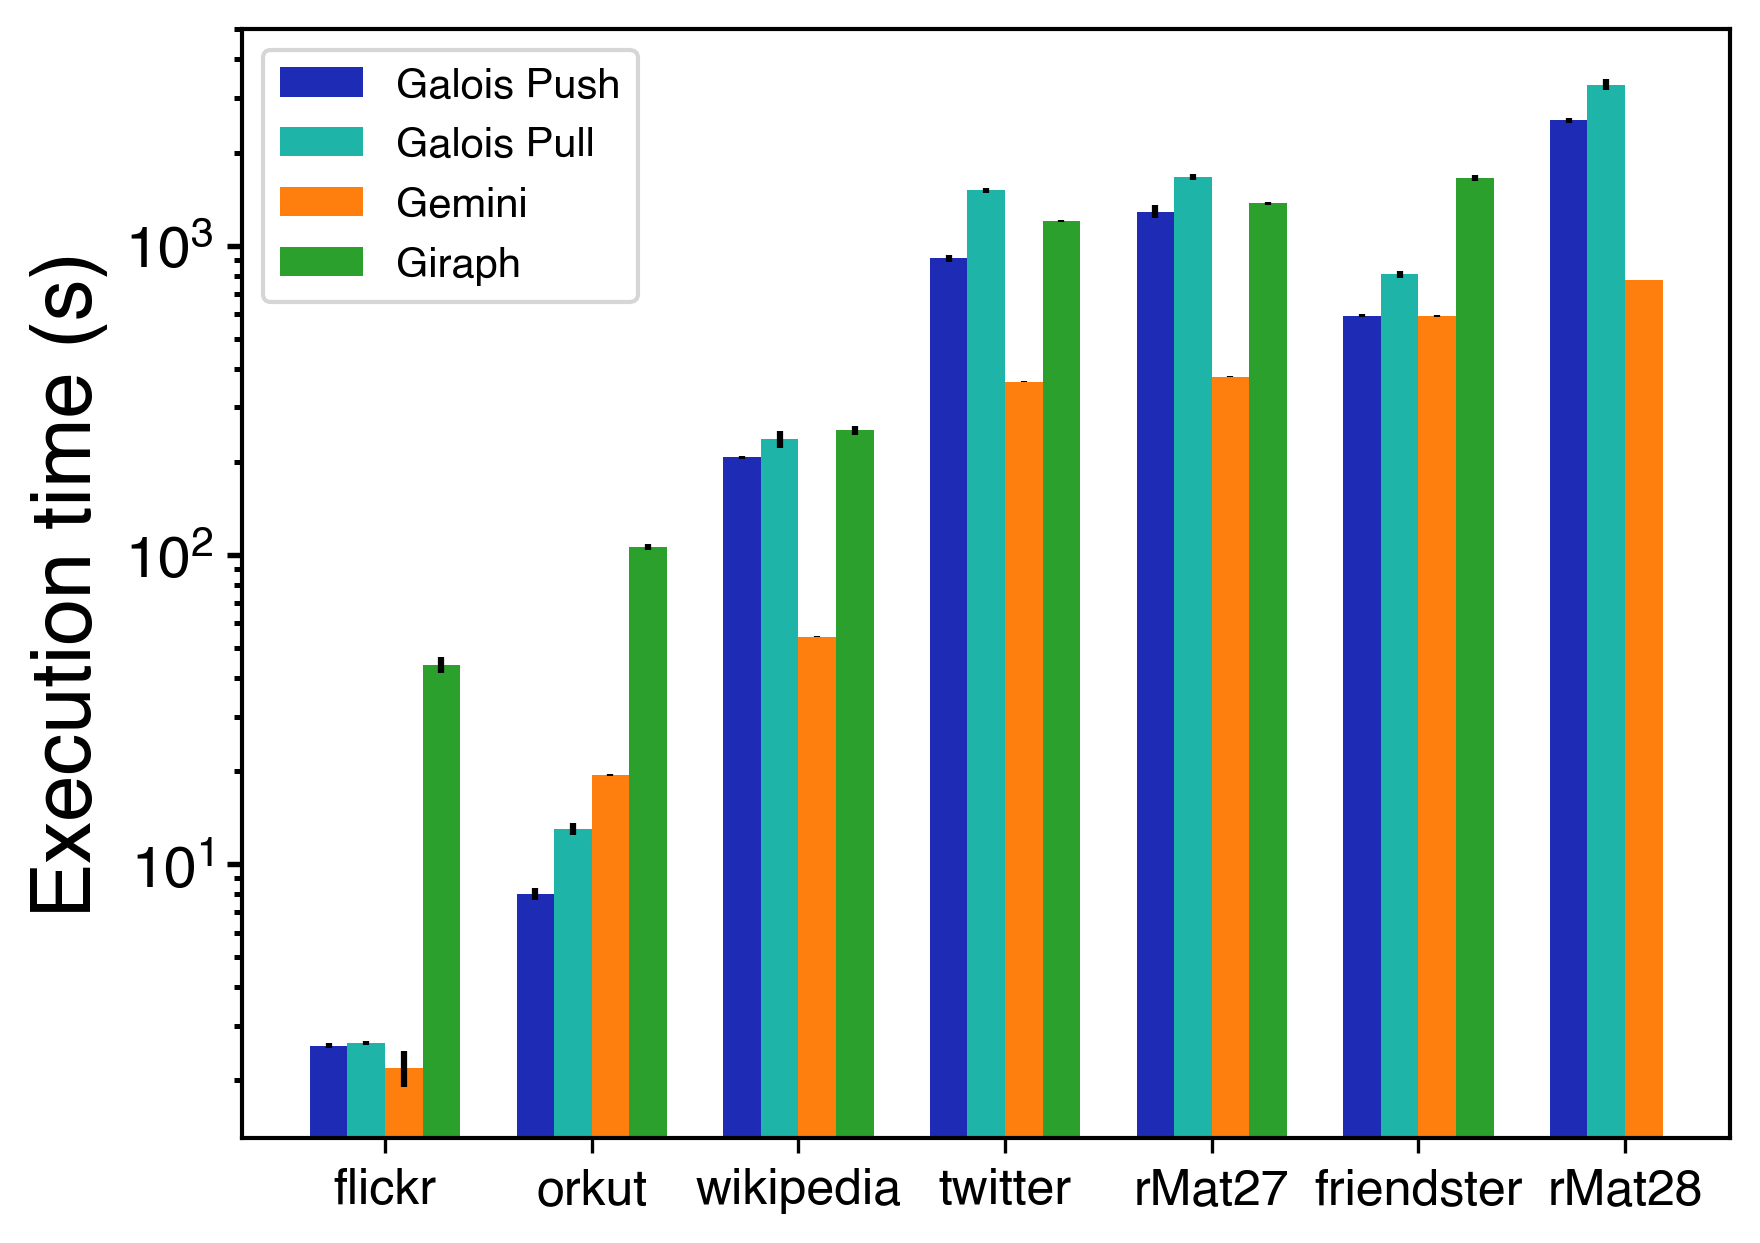
\includegraphics[width=\linewidth]{../../plots/distributedPR_execTime.png}
		\caption{PR}
		\label{fig:distributedSSSP_exec}
	\end{subfigure}
\end{figure}
\begin{itemize}
	\item Galois Push is faster than Pull in all cases
	\item Both Galois implementations fastest on SSSP or BFS
	\item Gemini is fastest on PR in almost all cases
\end{itemize}


%\newgeometry{paperwidth=28.1cm, paperheight=18cm, left=1cm, right=1cm, top=0.7cm,bottom=1cm,includefoot,heightrounded}
\section{Galois With Hugepages}
\begin{figure}[h!]
\begin{subfigure}{0.4\textwidth}
	\sffamily
	\small
	\centering
	\begin{tabular}{cr@{\tabskip 2 \tabcolsep}rr@{\tabskip 2 \tabcolsep}r}
		&\multicolumn{2}{c}{\bf Calc Time (s)}&\multicolumn{2}{c}{\bf Exec Time (s)}\\
		\cmidrule{2-3}\cmidrule{4-5}
		\bf Graph&w/o&w/&w/o&w/\\
		\midrule
		flickr & 0.01 & \bf 0.01 & 0.3 & \bf 0.2\\
		orkut & 0.10 & \bf 0.02 & 0.8 & \bf 0.5\\
		wikipedia & 0.38 & \bf 0.11 & 1.8 & \bf 1.1\\
		twitter & 2.47 & \bf 0.94 & 10.8 & \bf 5.1\\
		rMat27 & 4.50 & \bf 1.39 & 16.0 & \bf 6.4\\
		friendster & 4.70 & \bf 1.78 & 14.4 & \bf 7.5\\
		rMat28 & 9.77 & \bf 3.34 & 27.8 & \bf 13.1\\
\end{tabular}
\caption{SSSP}
\end{subfigure}
\hfil
\begin{subfigure}{0.4\textwidth}
\sffamily
\small
\centering
\begin{tabular}{cr@{\tabskip 2 \tabcolsep}rr@{\tabskip 2 \tabcolsep}rc}
		&\multicolumn{2}{c}{\bf Calc Time (s)}&\multicolumn{2}{c}{\bf Exec Time (s)}\\
		\cmidrule{2-3}\cmidrule{4-5}
		\bf Graph&w/o&w/&w/o&w/\\
		\midrule
		flickr & 0.01 & \bf 0.01 & 0.3 & \bf 0.2\\
		orkut & 0.06 & \bf 0.02 & 0.7 & \bf 0.6\\
		wikipedia & 0.17 & \bf 0.03 & 1.7 & \bf 1.4\\
		twitter & 0.77 & \bf 0.11 & \bf 8.7 & 9.3\\
		rMat27 & 0.65 & \bf 0.13 & 19.2 & \bf 8.1\\
		friendster & 1.01 & \bf 0.14 & 20.4 & \bf 13.1\\
		rMat28 & 1.15 & \bf 0.24 & 46.0 & \bf 16.4\\
\end{tabular}
\caption{PR Pull}
\end{subfigure}
\end{figure}
\vfill
\begin{itemize}
	\item Hugepages reduce both calculation and execution time on all algorithms
	\item[$\rightarrow$] Execution times can be up to 3$\times$ shorter
\end{itemize}
\vfill


\section{Multithreaded Speedup of Galois}
\begin{figure}[h!]
\begin{subfigure}{0.45\textwidth}
	\centering
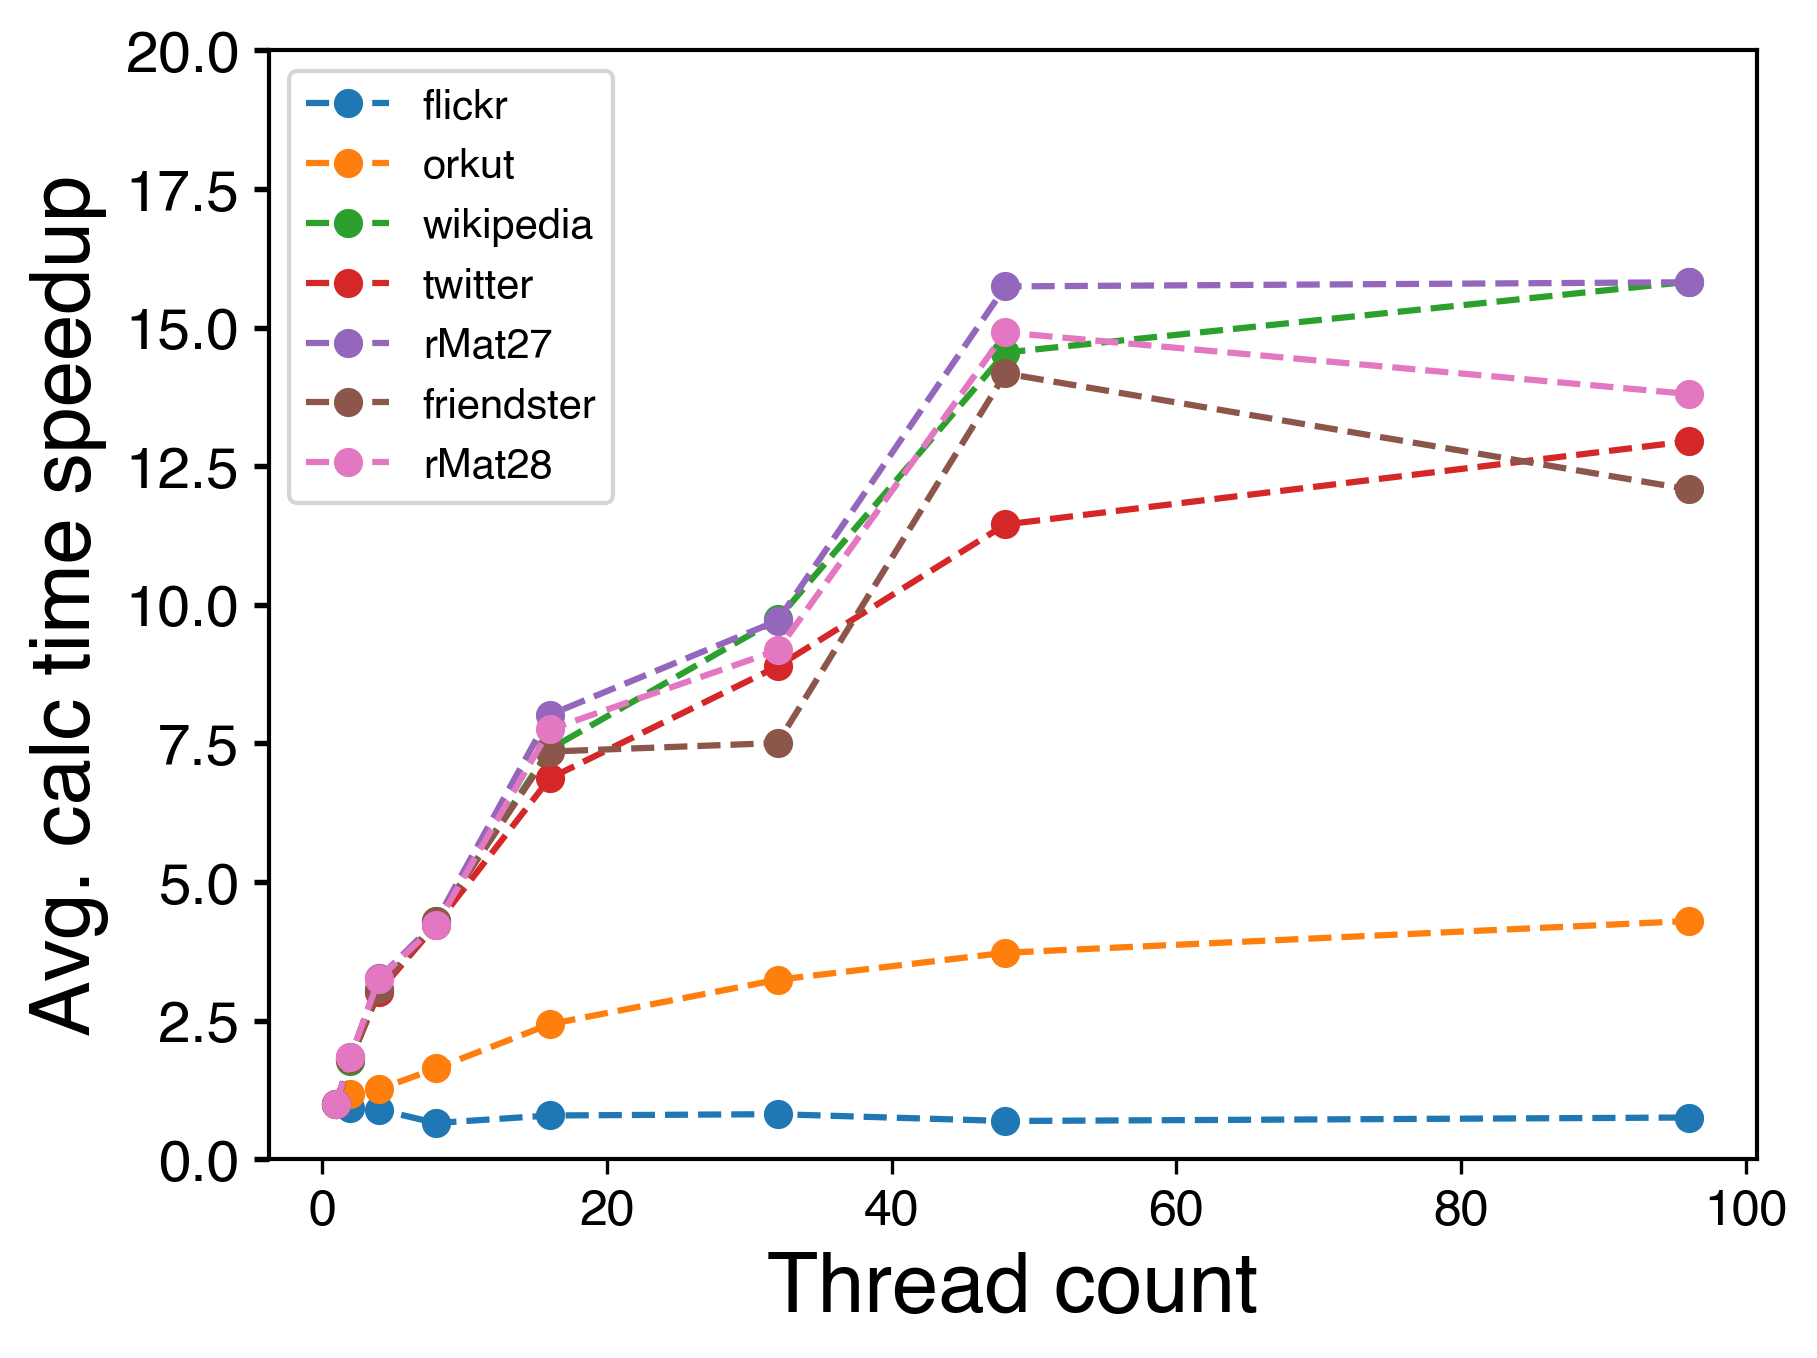
\includegraphics[width=\linewidth]{../../plots/singleNodeSSSPGaloisHPThreads.png}
\caption{SSSP with Hugepages}
\end{subfigure}
\hfil
\begin{subfigure}{0.45\textwidth}
	\centering
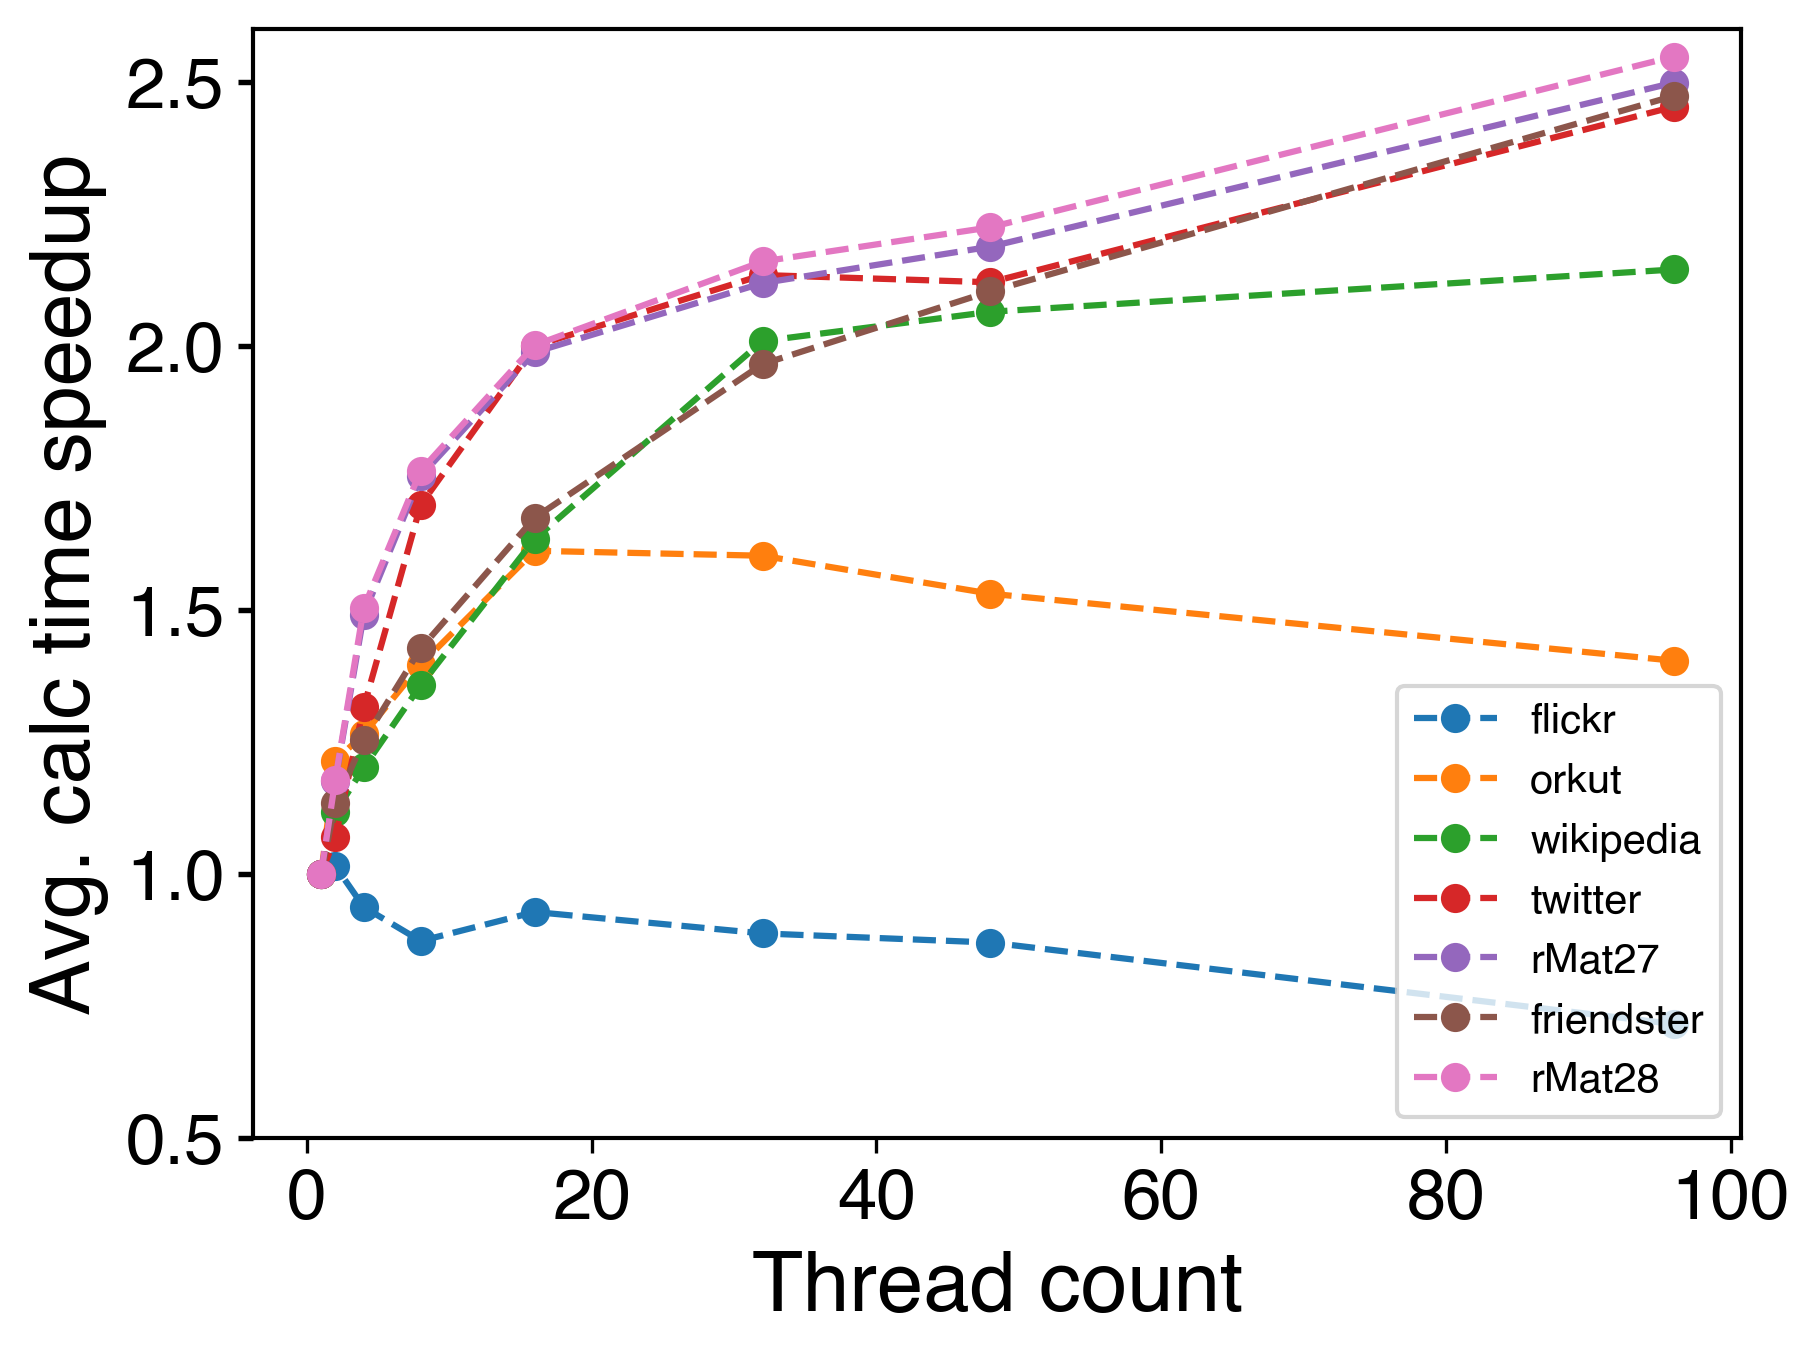
\includegraphics[width=\linewidth]{../../plots/singleNodePRPullGaloisHPThreads.png}
		\caption{PR Pull with Hugepages}
	\end{subfigure}
\end{figure}
\begin{itemize}
	\item Speedups can be significant, with and without hugepages
	\item Speedup of PR not to the same degree as on SSSP (2.5$\times$ vs. 15$\times$)
\end{itemize}


\restoregeometry



\section{Conclusion and Outlook}
Generally: 1) performance highly dependent on the framework, algorithm and data set

2) single node almost always preferrable, as long as RAM is sufficient
\begin{multicols}{2}
	\subsection{Production Case}
	\begin{itemize}
		\item Giraph is very fast on distributed systems (especially SSSP and BFS)
		\item Gemini is fast for distributed PR
		\item Gemini and Ligra are good options for single node 
	\end{itemize}

	\columnbreak
	\subsection{Research Case}
	\begin{itemize}
		\item Galois is fastest in almost all cases; further improvements with hugepages possible
	\end{itemize}
\end{multicols}


\subsection{Outlook}
\begin{itemize}
	\item[$\rightarrow$] incorporate new frameworks and new algorithms
	\item[$\rightarrow$] explore range of settings and other implementations
	\item[$\rightarrow$] repeat similar tests in the future: frameworks are updated and new ones are introduced
\end{itemize}





\end{document}
